% ---------------------------------------------------------------------------------------
\chapter{Comprarando una Imgaen con su tranformada}\label{chap5}

\section{Introducci\'on}

    Como ya mencionamos en el cap\'itulo \ref{chap4} se utilizaron im\'agenes de la base de datos ''\textit{Kodak Lossless TrueColor Image Suite}''\ref{fig:rgb2gray_2} \cite{KodakLosslessTrueColorImageSuite}. A cada una de las correspondientes im\'agenes ser\'an pasadas a blanco y negro, como fue descrito en \ref{eq:grayscale}, y posteriormente se le aplicar\'a la transformaci\'on de Box-Cox con los tr\'es m\'etodos de selecci\'on de $\lambda$ descritos en el cap\'itulo anteror.

    \begin{figure}[H]
        \centering
        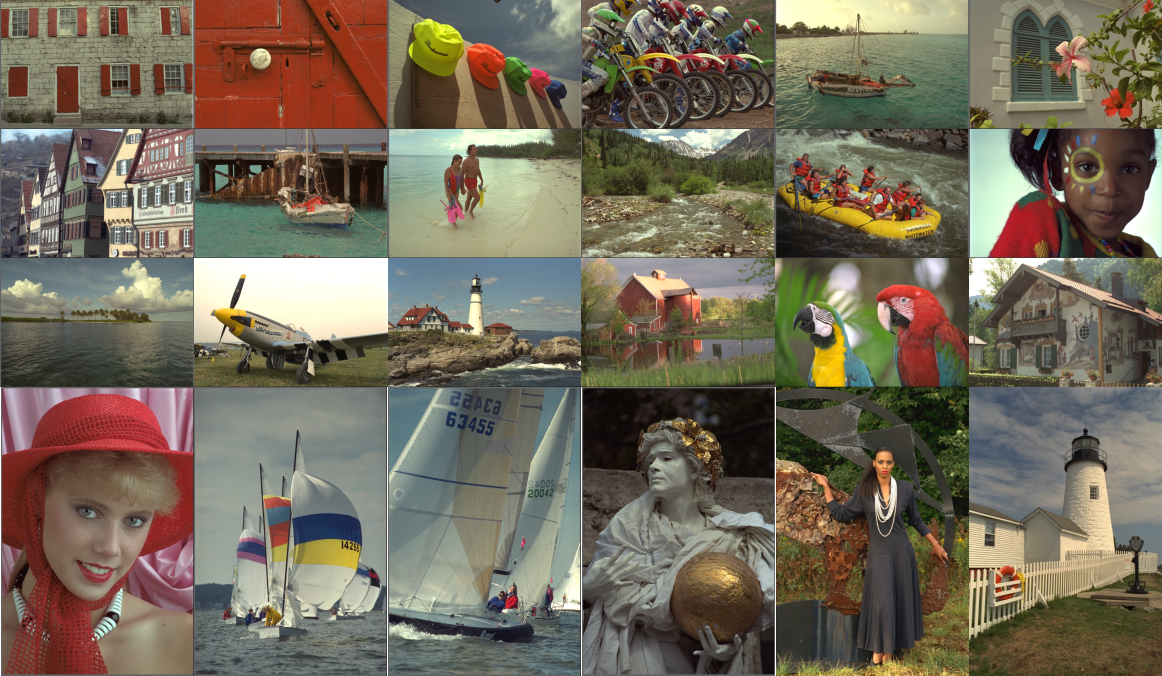
\includegraphics[width=0.5\textwidth]{all_images_grid.png}
        \caption{Banco de imagenes en blanco y negro.}
        \label{fig:rgb2gray_2}
    \end{figure}
    
    Ya revisamos el efecto que en general tiene cada $\lambda$ en la im\'agen, y como la selecci\'on de este afecta a cada una, en la siguientes secci\'ones discutiremos la relaci\'on que existe entre una im\'agen y su transformada para $\lambda$ cualquiera en el conjunto $[-2, 5]\subset\R$ y posteriormente como se ve la relaci\'on entre una im\'agen y su transformada usando los distintos lamdba entregados 
    
\section[Comparando imagenes vs. lambda]{Comparando imagenes vs. $\lambda$}

    Antes de comparar las im\'agenes con su tranformada dado el $\lambda$ eleguido por algunos de los m\'etodos estudiados, queremos revisar si hay una relaci\'on com\'un entre las im\'agnes y su transformada para un $\lambda$ cualquiera en $[-2, 5]\subset\R$. Veamos los resultados \todo{ref figura, crear una solo figura con todo}. Veamos primero los resultados sobre las im\'agenes completas


    \begin{figure}[H]
        \centering
        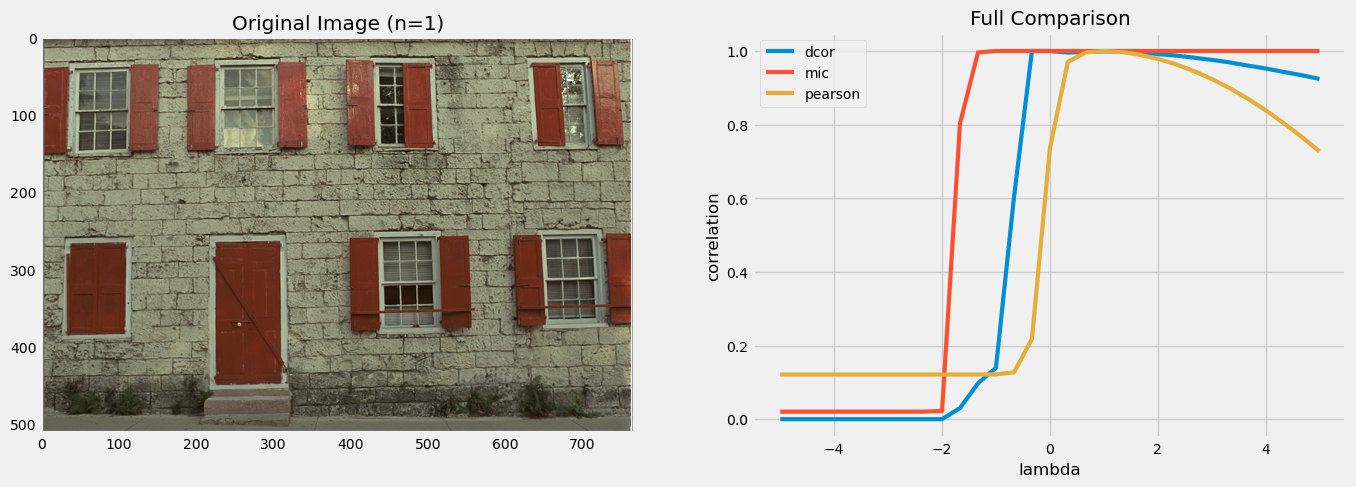
\includegraphics[width=0.5\textwidth]{lam_v_com_1.png}
        \caption{Im\'agen 1 junto con su correlaci\'on vs. $\lambda$}
    \end{figure}

    \begin{figure}[H]
        \centering
        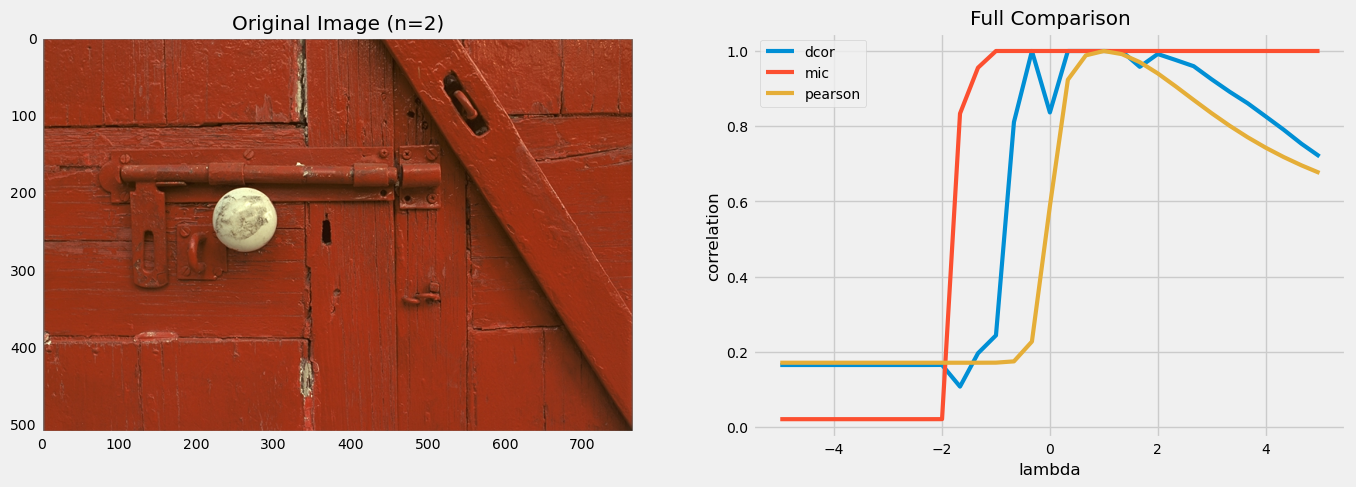
\includegraphics[width=0.5\textwidth]{lam_v_com_2.png}
        \caption{Im\'agen 2 junto con su correlaci\'on vs. $\lambda$}
    \end{figure}

    \begin{figure}[H]
        \centering
        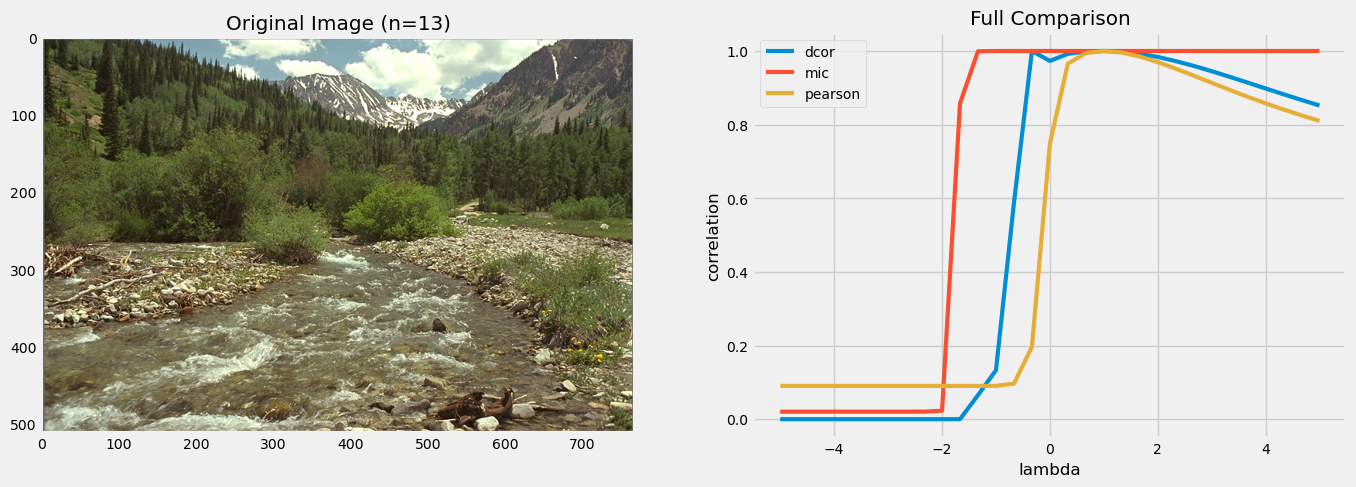
\includegraphics[width=0.5\textwidth]{lam_v_com_13.png}
        \caption{Im\'agen 13 junto con su correlaci\'on vs. $\lambda$}
    \end{figure}

    \begin{figure}[H]
        \centering
        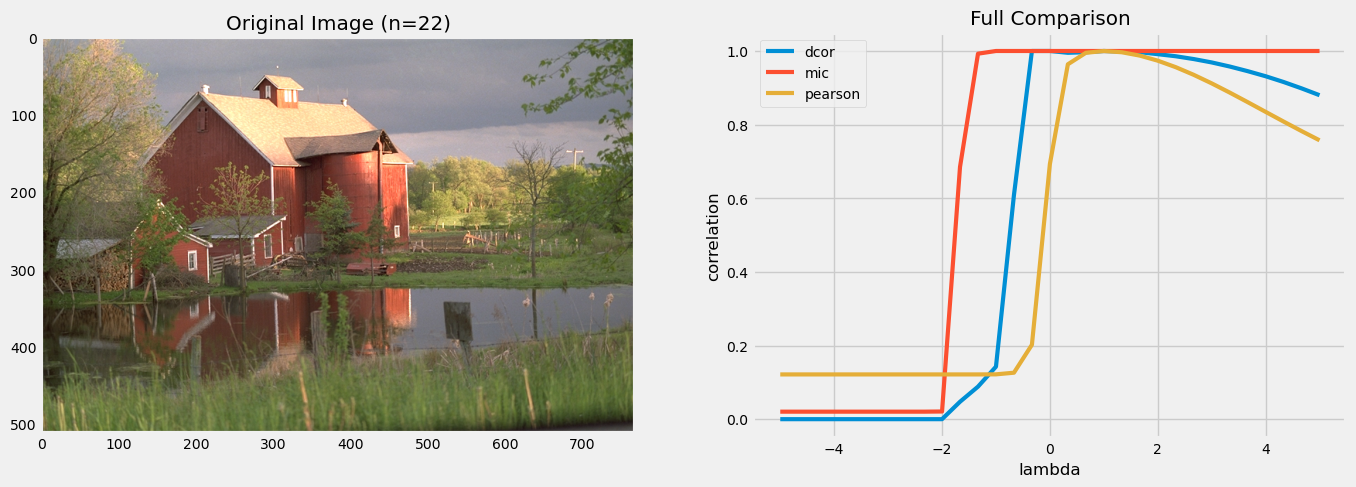
\includegraphics[width=0.5\textwidth]{lam_v_com_22.png}
        \caption{Im\'agen 22 junto con su correlaci\'on vs. $\lambda$}
    \end{figure}

    Podemos ver que todas las curvas se comportan de forma similar, pero cabe descatar que el el MIC el cual detecta la relaci\'on de forma m\'as temprana, con dCor siguiendo no mucho m\'as atr\'as. Otra cosa que vale la pena mencionar es que el MIC mantiene una correlaci\'on alta con la im\'agen original, incluso para valores altos de $\lambda$, cosa que no ocurre con dCor, el cual disminuyemientas los valores de $\lambda$ van aumentando.

    Repitiendo lo anterior, pero ahora con el m\'etodo del histograma tenemos: 

    \begin{figure}[H]
        \centering
        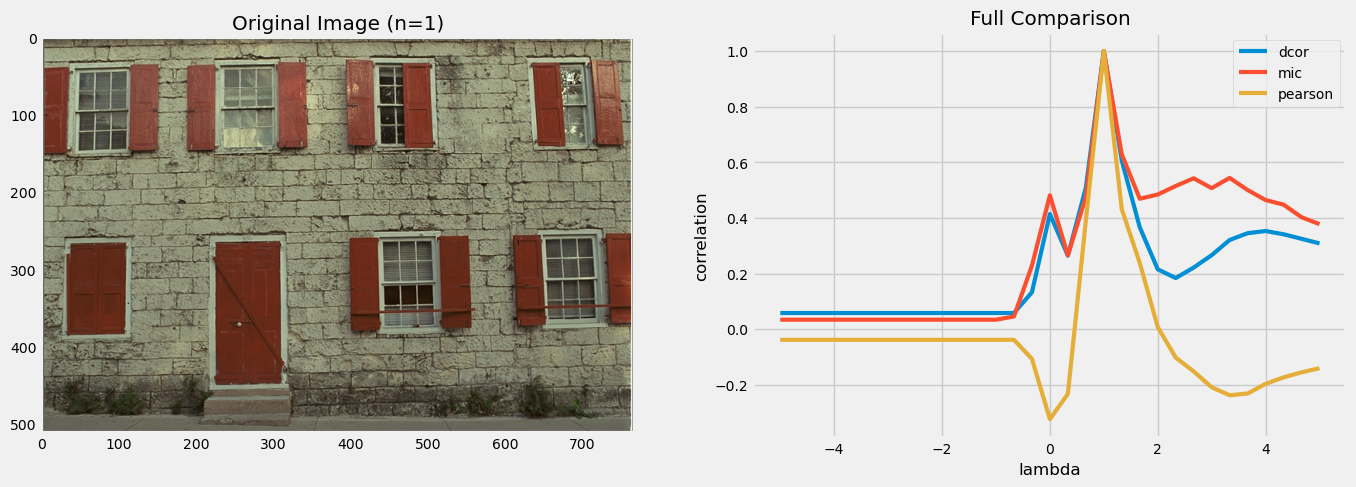
\includegraphics[width=0.5\textwidth]{lam_v_com_1_hist.png}
        \caption{Im\'agen 1 junto con su correlaci\'on vs. $\lambda$}
    \end{figure}

    \begin{figure}[H]
        \centering
        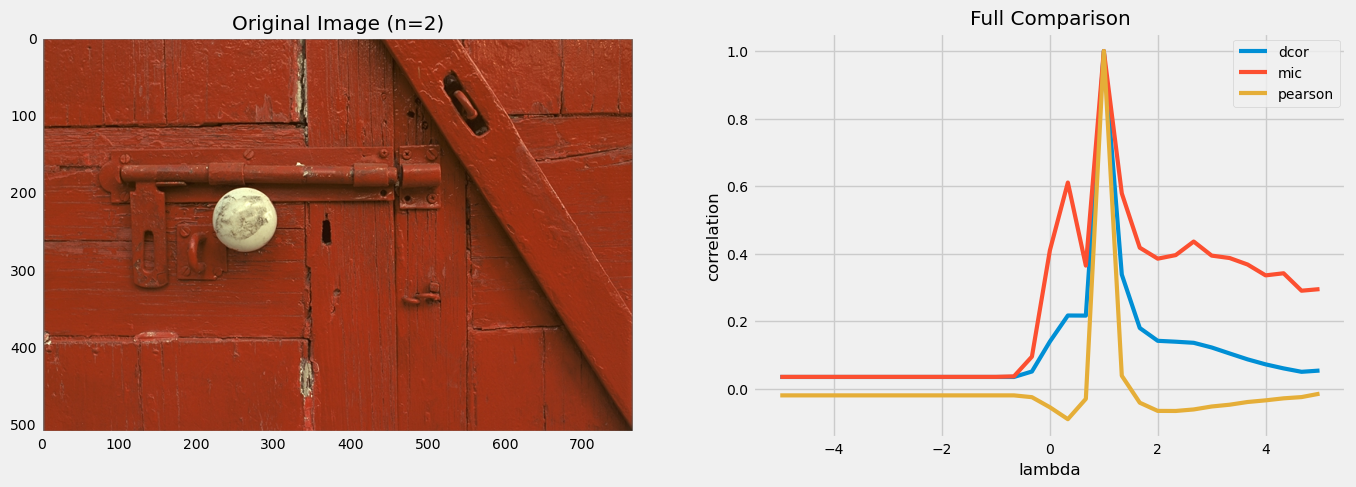
\includegraphics[width=0.5\textwidth]{lam_v_com_2_hist.png}
        \caption{Im\'agen 2 junto con su correlaci\'on vs. $\lambda$}
    \end{figure}

    \begin{figure}[H]
        \centering
        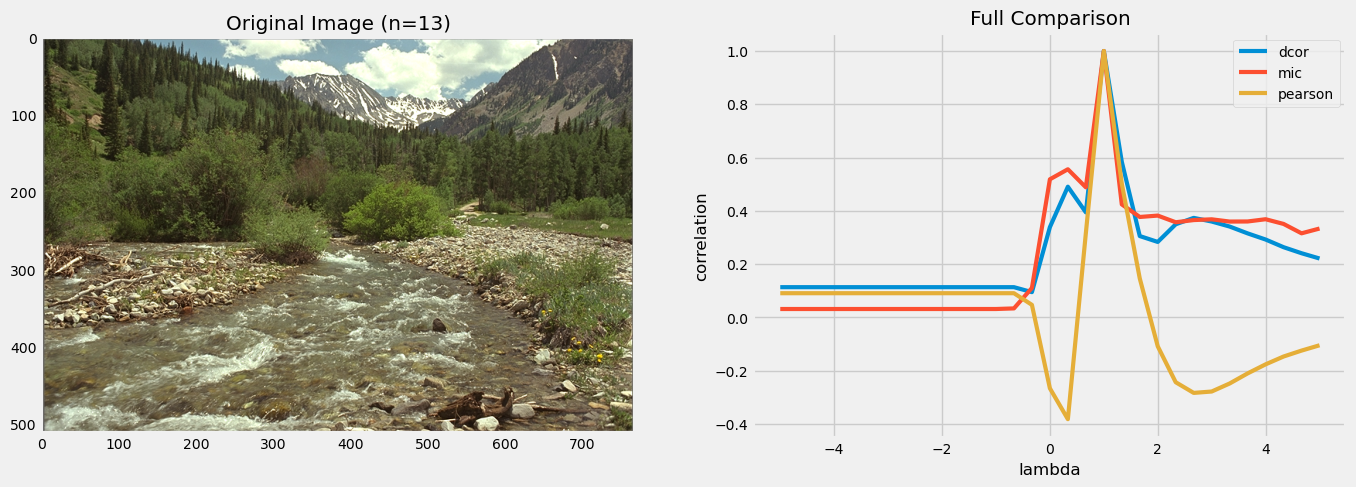
\includegraphics[width=0.5\textwidth]{lam_v_com_13_hist.png}
        \caption{Im\'agen 13 junto con su correlaci\'on vs. $\lambda$}
    \end{figure}

    \begin{figure}[H]
        \centering
        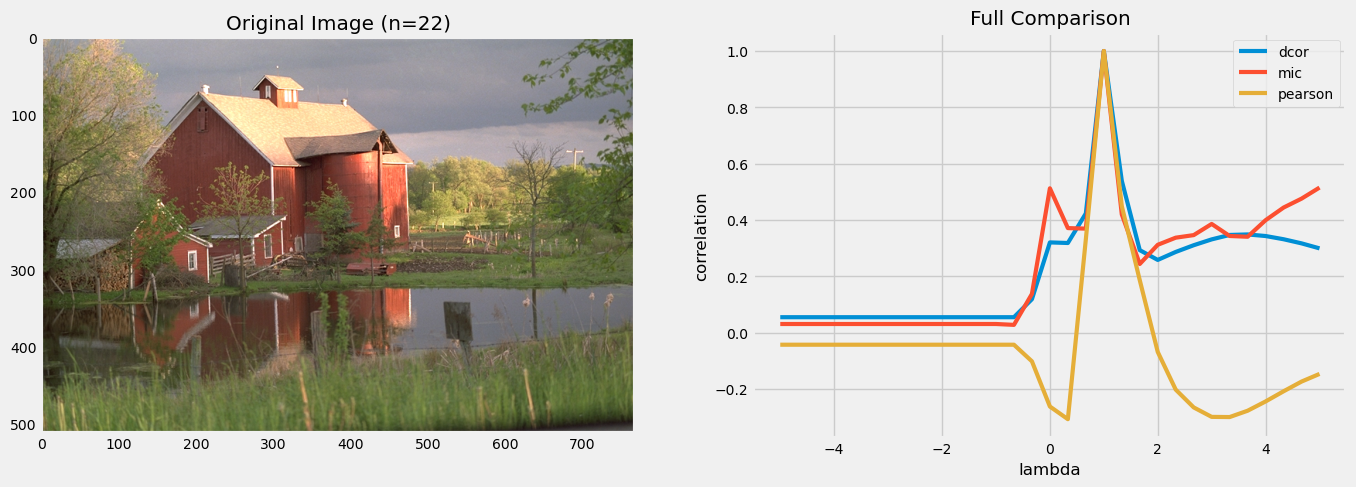
\includegraphics[width=0.5\textwidth]{lam_v_com_22_hist.png}
        \caption{Im\'agen 22 junto con su correlaci\'on vs. $\lambda$}
    \end{figure}

    Podemos ver que tenemos un efecto similar, \todo{ampliar conclusion}



\section{Comparando imagenes con su tranformada}
todo{necesita un mejor titulo}

    \todo{todo esto}

    Esta es la parte en la que comparamos el valor de la correlaci\'on entre la im\'agen y su transformada para cada m\'etodo de selecci\'on de $\lambda$. 

    Es en donde m\'as dudas tengo sobre concluir, que mencionar, etc. dejo un resumen de los resultados y quedo atento a los compentarios
    
    Al comparar las imagenes suando sus histogramas obtener los siguientes promedios (full, hist y grid se refieren al m\'etodo de selecci\'on de $\lambda$)

    \begin{table}[H]
        \begin{tabular}{ll}
        mic\_full     & 0.483314  \\
        dcor\_full    & 0.453417  \\
        mic\_hist     & 0.450874  \\
        dcor\_hist    & 0.424125  \\
        mic\_grid     & 0.409863  \\
        dcor\_grid    & 0.357291  \\
        pearson\_full & 0.161884  \\
        pearson\_grid & 0.114137  \\
        pearson\_hist & -0.233827 \\
        pearson\_hist & -0.233827
        \end{tabular}
    \end{table}

    noteamos que la mayor relacion la encontramos al usar toda la imagen parabuscar un lamdba

    en el caso de comparar las imagenes usando todo el vector, tenemos

    \begin{table}[H]
        \begin{tabular}{ll}
        dcor\_full    & 1.000000  \\
        mic\_full     & 1.000000  \\
        mic\_hist     & 1.000000  \\
        pearson\_full & 0.987437  \\
        mic\_grid     & 0.970955  \\
        dcor\_hist    & 0.947233  \\
        pearson\_hist & 0.924601  \\
        pearson\_hist & 0.924601  \\
        dcor\_grid    & 0.865844  \\
        pearson\_grid & 0.842625  \\
        pearson\_hist & -0.233827
        \end{tabular}
    \end{table}

    en donde vemos que la mayor relaci\'on la encontramos al usar todo el vector para buscar un $\lambda$, pero no es muy distinto a usar el histograma.

    En general usar grid para buscar un $\lambda$ es el peor m\'etodo, pero no es muy distinto a usar el histograma.

    Veamos como se ven los valores para cada imagen, primero comparando los histogramas y luego comparando todo el vector

    \begin{figure}[H]
        \centering
        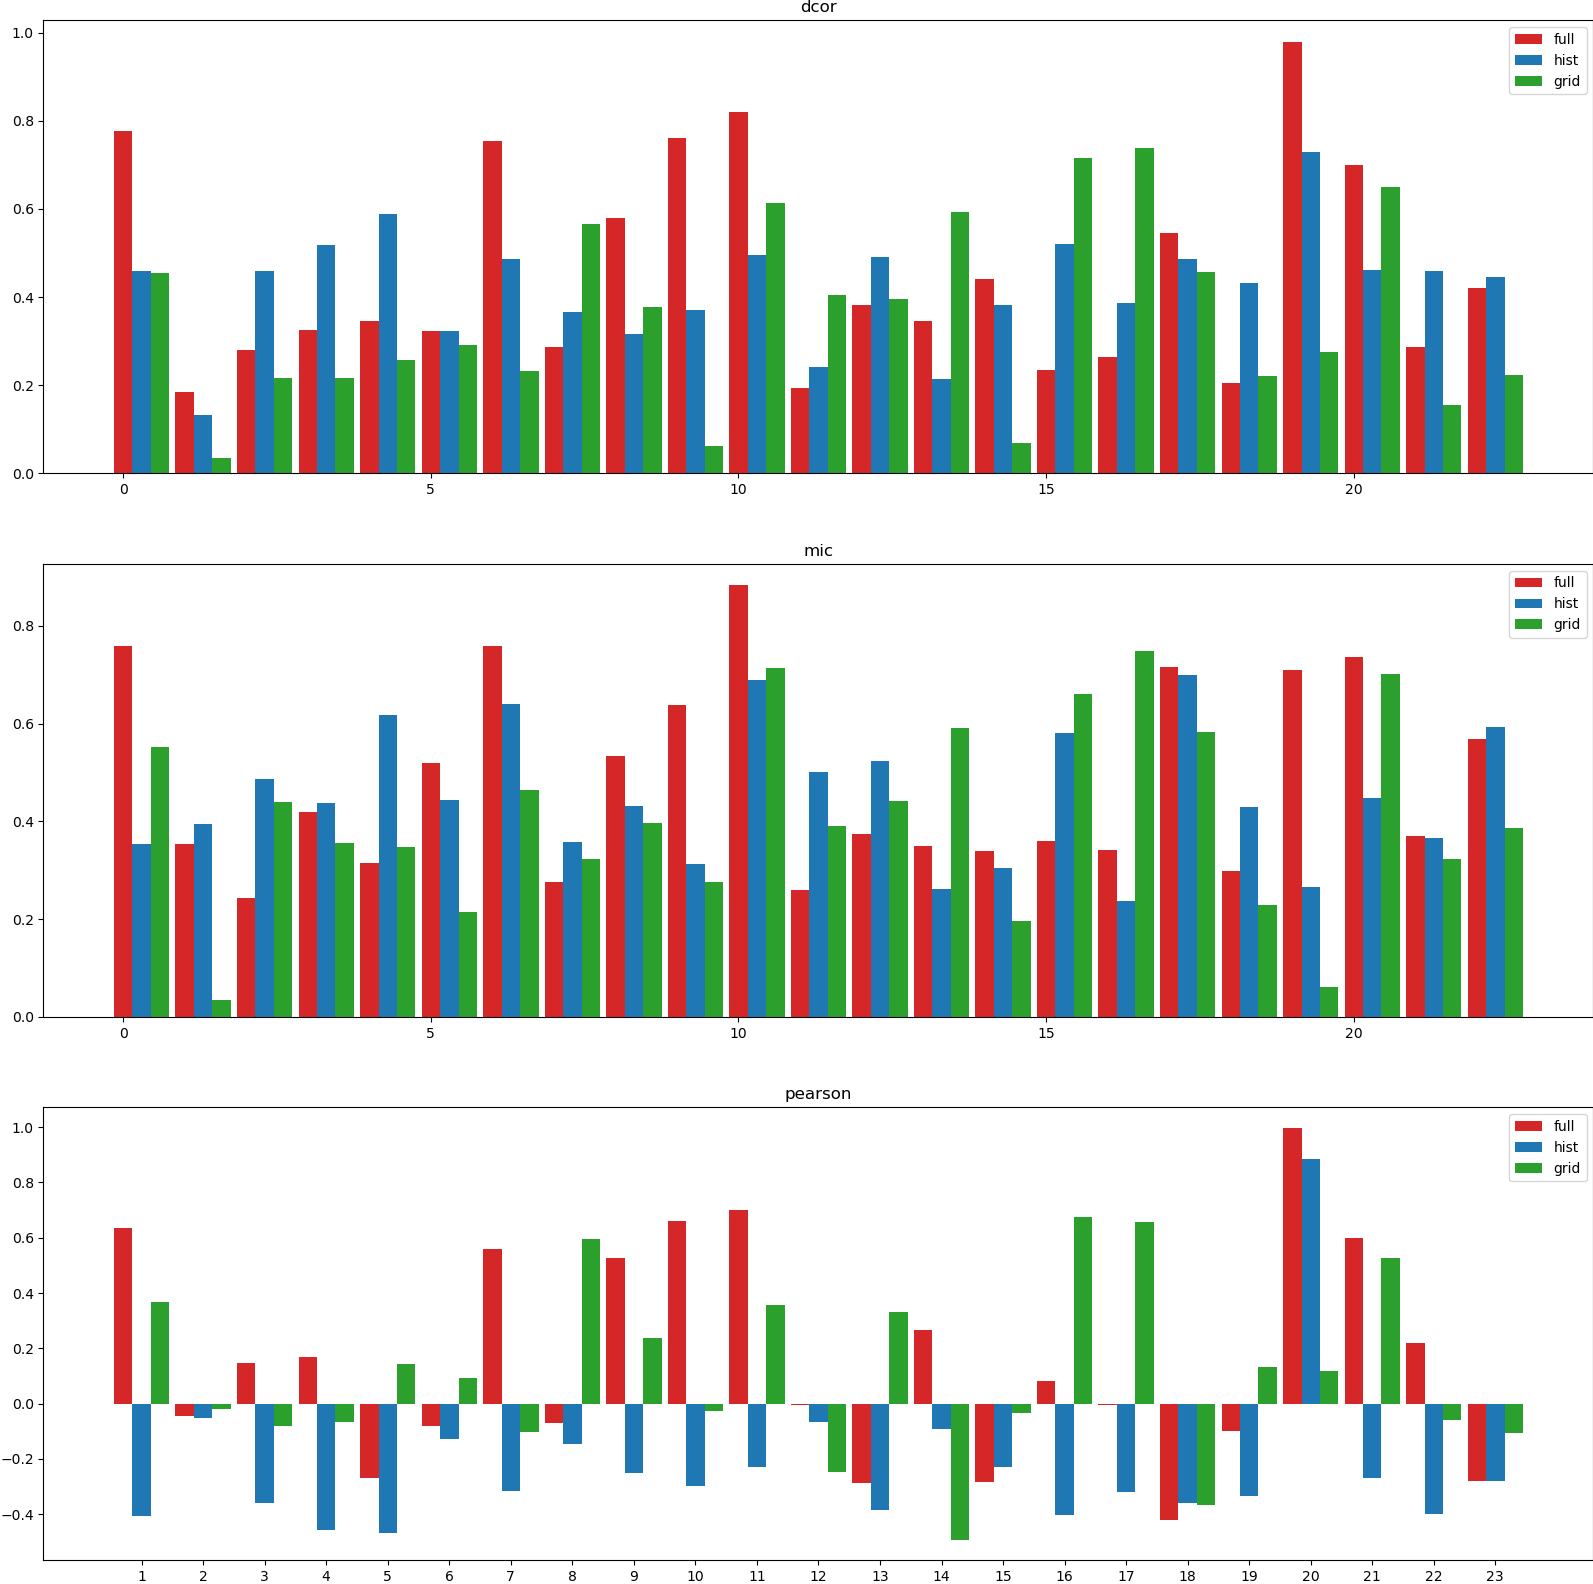
\includegraphics[width=0.6\textwidth]{plot_comparison_hist.png}
        \caption{Valores de dcor, mic y pearson para cada imagen usando el histograma, azul es el metodo para encontrar $\lambda$ con toda la imagen, rojo es el histograma y amarillo es el grid}
    \end{figure}


    \begin{figure}[H]
        \centering
        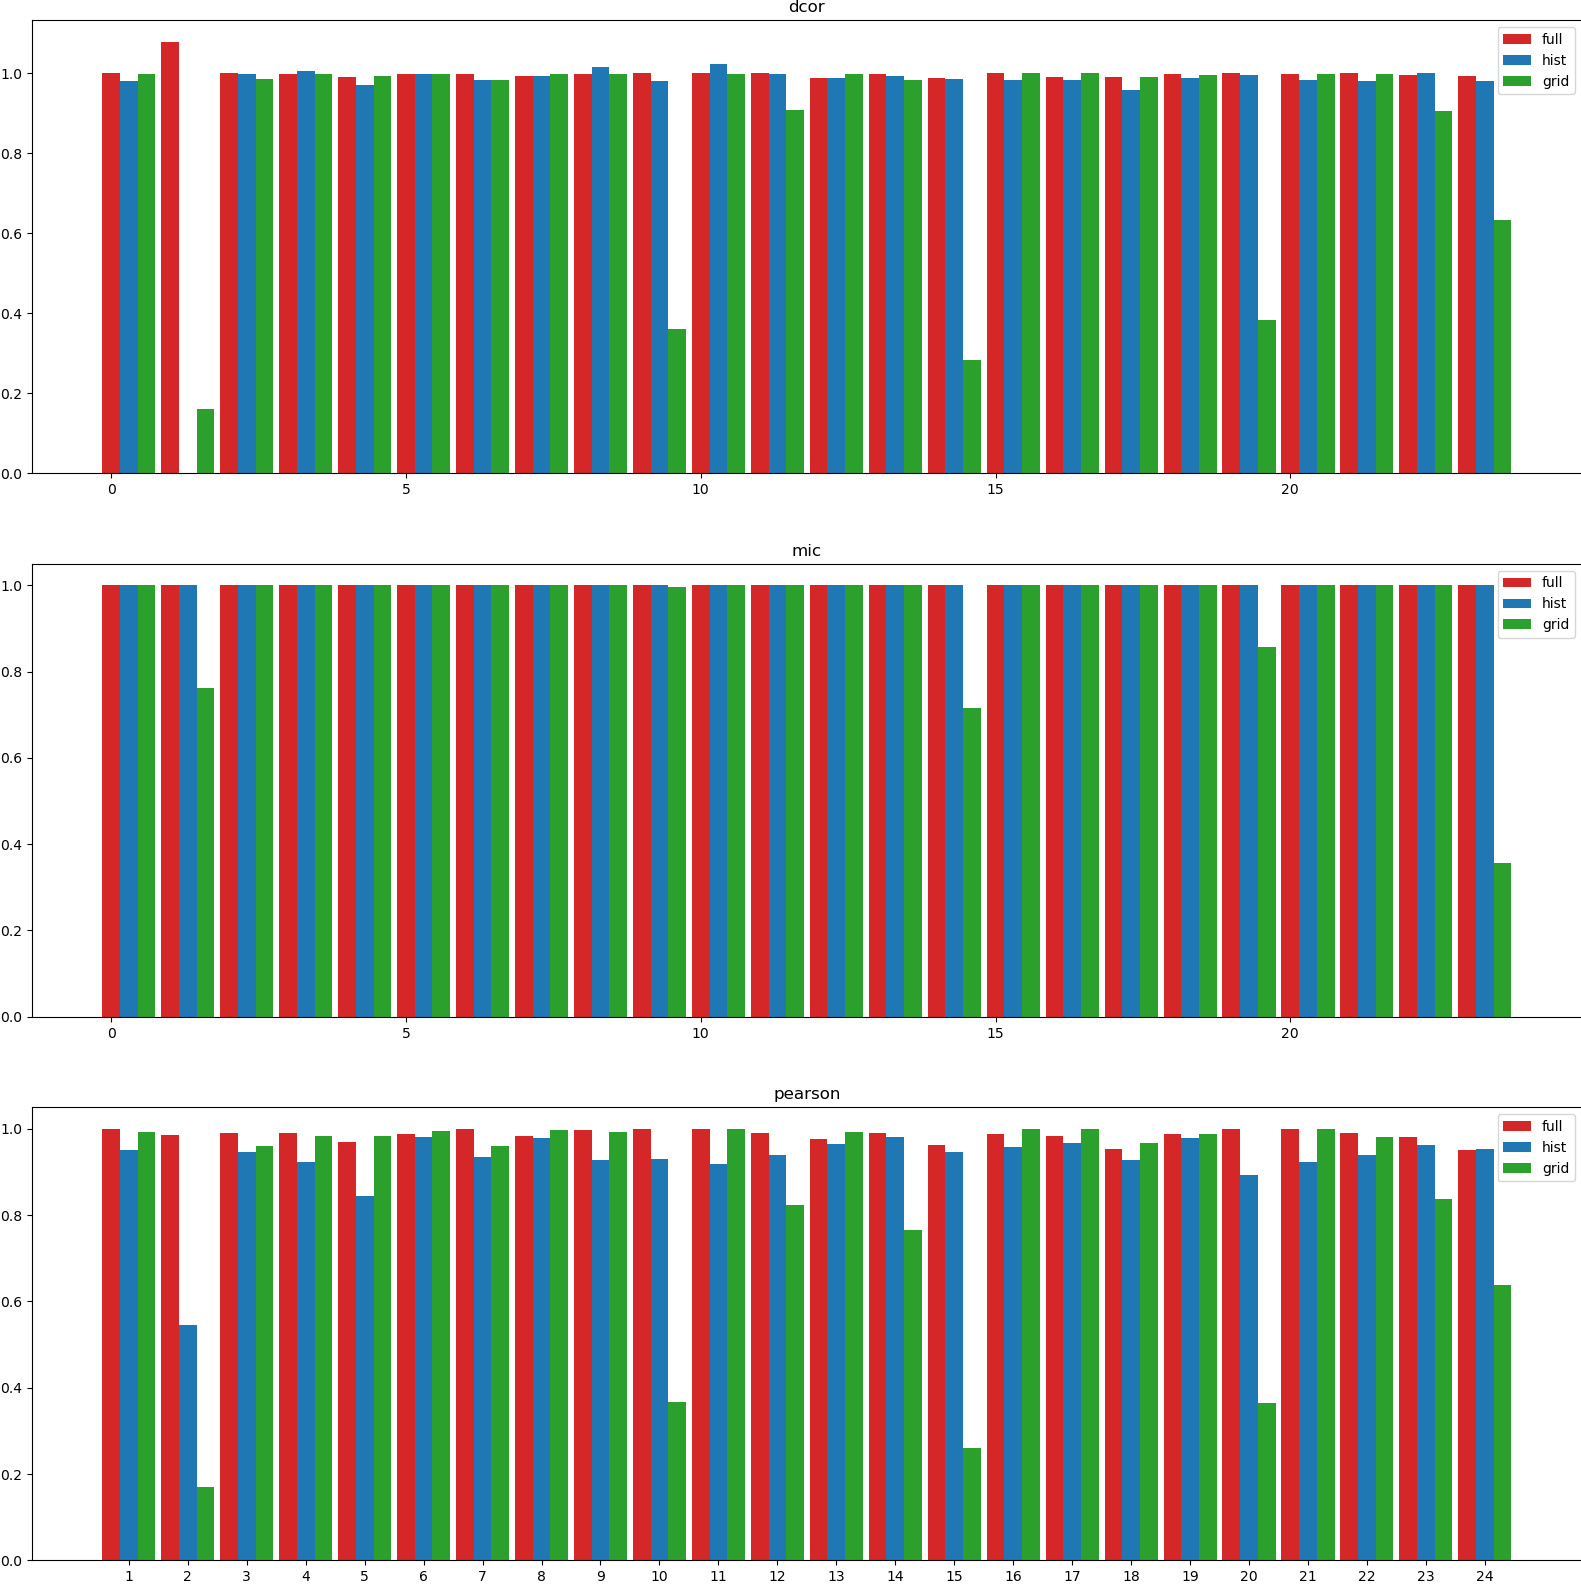
\includegraphics[width=0.6\textwidth]{plot_comparison_full.png}
        \caption{Valores de dcor, mic y pearson para cada imagen usando todo el vector, azul es el metodo para encontrar $\lambda$ con toda la imagen, rojo es el histograma y amarillo es el grid}
    \end{figure}

\section{Concluciones}

\todo{concluir}